\documentclass[11pt]{article}

% some definitions for the title page
\newcommand{\reporttitle}{Introduction Lecture for NLP and some ML baselines}
\newcommand{\reportdescription}{THe introductory lecture for Natural Language Processing and some core concepts for Natural Language Processing with supplementary material regarding basic ML concepts required for this course}

% load some definitions and default packages
%---------------------------------------------------------------------------
%	PACKAGES AND OTHER DOCUMENT CONFIGURATIONS
%---------------------------------------------------------------------------

\usepackage[twoside]{fancyhdr}
\usepackage{csquotes}

\usepackage[a4paper,hmargin=2.0cm,vmargin=1.0cm,includeheadfoot]{geometry}
% \usepackage{natbib} % for bibliography
\usepackage{biblatex}
\usepackage{tabularx,longtable,multirow,subfigure,caption}%hangcaption
\usepackage{fancyhdr} % page layout
\usepackage{url} % URLs
\usepackage[english]{babel}
\usepackage{graphicx}
\usepackage{rotating}
\usepackage{dsfont}
\usepackage{epstopdf} % automatically replace .eps with .pdf in graphics
% \usepackage{backref} % needed for citations
\usepackage{array}
\usepackage{latexsym}
\usepackage[pdftex,hypertexnames=false,colorlinks]{hyperref} % provide links in pdf (had pagebackref)
\usepackage{booktabs}
\usepackage{wrapfig}
\usepackage{caption}  % Required for \captionof
\usepackage{float} % for H option in figures
\usepackage{amssymb}
\usepackage{amsmath}
\usepackage{amsthm}
\usepackage{mathtools} % for 'dcases*' env.
\usepackage[nottoc]{tocbibind}

%%% Default fonts
\renewcommand*{\rmdefault}{bch}
\renewcommand*{\ttdefault}{cmtt}

%%% Default settings (page layout)
\setlength{\parindent}{0em}  % indentation of paragraph
\setlength{\parskip}{.3em}
\setlength{\itemsep}{0.mm}

\setlength{\headheight}{14.5pt}
\pagestyle{fancy}

\fancyfoot[ER,OL]{\thepage}%Page no. in the left on odd pages and on right on even pages

\fancyfoot[OC,EC]{\sffamily }
\renewcommand{\headrulewidth}{0.1pt}
\renewcommand{\footrulewidth}{0.1pt}
\captionsetup{margin=10pt,font=small,labelfont=bf}

% LISTINGS ammendments
\usepackage{listings}
\usepackage{color}

\definecolor{mygreen}{rgb}{0,0.6,0}
\definecolor{mygray}{rgb}{0.5,0.5,0.5}
\definecolor{mymauve}{rgb}{0.58,0,0.82}

\lstset{ 
  postbreak=\mbox{\textcolor{red}{$\hookrightarrow$}\space},
  backgroundcolor=\color{white},   % choose the background color; you must add \usepackage{color} or \usepackage{xcolor}; should come as last argument
  basicstyle=\footnotesize,        % the size of the fonts that are used for the code
  breakatwhitespace=false,         % sets if automatic breaks should only happen at whitespace
  breaklines=true,                 % sets automatic line breaking
  captionpos=b,                    % sets the caption-position to bottom
  commentstyle=\color{mygreen},    % comment style
%   deletekeywords={...},            % if you want to delete keywords from the given language
%   escapeinside={\%*}{*)},          % if you want to add LaTeX within your code
  extendedchars=true,              % lets you use non-ASCII characters; for 8-bits encodings only, does not work with UTF-8
  firstnumber=1,                % start line enumeration with line 1000
  frame=single,	                   % adds a frame around the code
  keepspaces=true,                 % keeps spaces in text, useful for keeping indentation of code (possibly needs columns=flexible)
  columns=fullflexible,
  keywordstyle=\color{blue},       % keyword style
  language=python,                 % the language of the code
  % morekeywords={*,...},            % if you want to add more keywords to the set
  numbers=left,                    % where to put the line-numbers; possible values are (none, left, right)
  numbersep=5pt,                   % how far the line-numbers are from the code
  numberstyle=\tiny\color{mygray}, % the style that is used for the line-numbers
  rulecolor=\color{black},         % if not set, the frame-color may be changed on line-breaks within not-black text (e.g. comments (green here))
  showspaces=false,                % show spaces everywhere adding particular underscores; it overrides 'showstringspaces'
  showstringspaces=false,          % underline spaces within strings only
  showtabs=false,                  % show tabs within strings adding particular underscores
  stepnumber=1,                    % the step between two line-numbers. If it's 1, each line will be numbered
  stringstyle=\color{mymauve},     % string literal style
  tabsize=2,	                   % sets default tabsize to 2 spaces
  title=\lstname% show the filename of files included with \lstinputlisting; also try caption instead of title
}

% Here, you can define your own macros. Some examples are given below.

\newcommand{\R}[0]{\mathds{R}} % real numbers
\newcommand{\Z}[0]{\mathds{Z}} % integers
\newcommand{\N}[0]{\mathds{N}} % natural numbers
\newcommand{\C}[0]{\mathds{C}} % complex numbers
\renewcommand{\vec}[1]{{\boldsymbol{{#1}}}} % vector
\newcommand{\mat}[1]{{\boldsymbol{{#1}}}} % matrix


\bibliography{../bibliography}

\begin{document}

% Include the title page
\begin{titlepage}

    \newcommand{\HRule}{\rule{\linewidth}{0.5mm}} % Defines a new command for the horizontal lines, change thickness here
    
    \center % Center everything on the page
     
    %------------------------------------------------------------------------
    %	HEADING SECTIONS
    %------------------------------------------------------------------------
    
    \textsc{\Large Department of Computing}\\[0.5cm] 
    \textsc{\large Imperial College of Science, Technology and Medicine}\\[0.5cm] 
    
    %------------------------------------------------------------------------
    %	TITLE SECTION
    %------------------------------------------------------------------------
    
    \HRule \\[0.4cm]
    { \huge \bfseries \reporttitle}\\ % Title of your document
    \HRule \\[0.4cm]

    \textit{\reportdescription}
    
    \vspace{2em}

    %------------------------------------------------------------------------
    %	AUTHOR SECTION
    %------------------------------------------------------------------------
    
    \large \emph{Author: Anton Zhitomirskiy}

    \vspace{1em}

    \global\let\newpagegood\newpage
    \global\let\newpage\relax
    
\end{titlepage}

\global\let\newpage\newpagegood

\tableofcontents

\clearpage

\section{Dealing with natural language}

\subsection{Complexities}

\begin{itemize}
    \item Ambiguity at word level
          \begin{quote}
            ``Can you bring me the file''
        \end{quote}
    \item Syntactic ambiguity (prepositional phrase attachment ambiguity)
          \begin{quote}
            ``I saw the boy with a telescope''
        \end{quote}
    \item Semantic ambiguity
          \begin{quote}
            ``I haven't slept for 10 days''
            ``The rabbit is ready for lunch''
        \end{quote}
    \item Referential ambiguity
          \begin{quote}
            ``We gave the monkeys bananas because they were more than ready to eat.''
        \end{quote}
    \item Non-literal meaning
          \begin{quote}
            ``Call me a cab, it's raining cats and dogs''
        \end{quote}
\end{itemize}

\subsection{The role of Deep Learning}

\begin{itemize}
    \item The creation and maintenance of linguistic rules often is infeasible or impractical.
    \item We'd much rather learn functions from data instead of creating rules based on intuition.
    \item deep learning is very flexible, learnable framework fro representing information from many different modalities.
\end{itemize}

\subsection{Composites of Language}

\subsubsection{Lexicon - morphological analysis}

Definition: Words: segmentation, normalisation, morphology

\begin{enumerate}
    \item Word Segmentation (tokenization, decompounding): 
    \begin{quote}
        ``For example, most of what we are going to do with language relies on first separating out or tokenizing words from running text, the task of tokenization. English words are often separated from each other tokenization by whitespace, but whitespace is not always sufficient. ``New York'' and ``rock 'n' roll'' are sometimes treated as large words despite the fact that they contain spaces, while sometimes we'll need to separate ``I'm'' into the two words ``I and am''''~\cite{book-speech-and-language-processing}
    \end{quote}
    \item Word normalization (capitalization, acronyms, spelling variants)
    \item Lemmatisation (reduce to base form = valid word)
    \begin{quote}
        ``Another part of text normalization is lemmatization, the task of determining lemmatization that two words have the same root, despite their surface differences. For example, the words sang, sung, and sings are forms of the verb sing. The word sing is the common lemma of these words, and a lemmatizer maps from all of these to sing''~\cite{book-speech-and-language-processing}
    \end{quote}
    \item Stemming (reduce to root = not always valid word)
    \begin{quote}
        ``Stemming refers to a simpler version of lemmatization in which we mainly stemming just strip suffixes from the end of the word''~\cite{book-speech-and-language-processing}.
    \end{quote}
    \item Byte-pair encoding (BPE) and wordpieces
    \begin{quote}
        ``Instead of defining tokens as words (whether delimited by spaces or more complex algorithms), or as characters (as in Chinese), we can use our data to automatically tell us what the tokens should be''~\cite{book-speech-and-language-processing}.
    \end{quote}

    \begin{figure}[H]
        \centering
        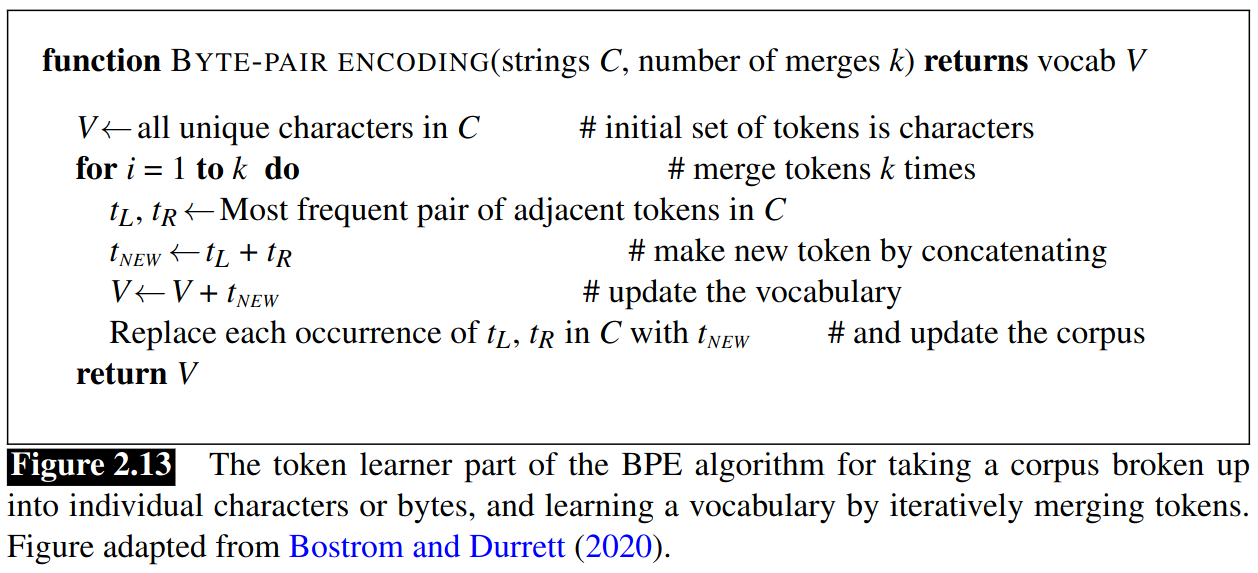
\includegraphics[width=.8\linewidth]{figures/bpe-algorithm.png}
        \label{fig:bpe-algorithm}
    \end{figure}

    \begin{quote}
        ``The BPE token learner begins BPE with a vocabulary that is just the set of all individual characters. It then examines the training corpus, chooses the two symbols that are most frequently adjacent (say 'A', 'B'), adds a new merged symbol 'AB' to the vocabulary, and replaces every adjacent 'A' 'B' in the corpus with the new 'AB'. It continues to count and merge, creating new longer and longer character strings, until k merges have been done creating k novel tokens; k is thus a parameter of the algorithm. The resulting vocabulary consists of the original set of characters plus k new symbols''~\cite{book-speech-and-language-processing}.
    \end{quote}

    \item Part-of-speech tagging (Recognize category of word): verb, noun, adverb, adjective, determiner, preposition... 
    
    It is the process of assigning a part-of-speech to each word in a text. This is a disambiguation task; words are ambiguous - have more tha one possible part-of-speech - and the goal is to find the correct tag for the sitauation. E.g. `book' can be a verb (`book that flight') or a noun (`hand me that book'). The POS-tagging resolves these ambiguities by choosing the proper tag for the context~\cite{book-speech-and-language-processing}.

    \item Morphological analysis (recognize/generate word variants):
    
    \begin{quote}
        ``Morphology is the study of the way words are built up from smaller meaning-bearing units called morphemes. Two broad classes of morphemes can be distinguished: \textbf{stems} — the central morpheme of the word, supplying the main meaning — and \textbf{affixes} — adding “additional” meanings of various kinds. So, for example, the word fox consists of one morpheme (the morpheme fox) and the word cats consists of two: the morpheme cat and the morpheme `-s'''~\cite{book-speech-and-language-processing}
    \end{quote}
\end{enumerate}

\subsubsection{Syntax}

Syntax comes from the Greek s'yntaxis, meaning “setting out together or arrangement”, and refers to the way words are arranged together~\cite{book-speech-and-language-processing}.

We can form a parse tree based on some syntax rules which makes up grammar. This was typically used in applications before deep learning; there are sentences that make sense but don't follow grammar.

\begin{tabular}{l c r}
    \hline
    \multicolumn{2}{c}{\textbf{Phrase Structure Rule}} & \textbf{Example} \\
    \hline
    $S \rightarrow NP \quad VP$ & Sentence $\rightarrow$ Noun-phrase Verb-phrase & I prefer a morning flight \\
    $NP \rightarrow Det\ N$ & Noun-phrase $\rightarrow$ Determiner Noun & prefer a morning flight\\
    $VP \rightarrow V NP$ & Verb-phrase $\rightarrow$ Verb Noun-phrase & leave Boston in the morning\\
    $VP \rightarrow V$ & Verb-phrase $\rightarrow$ Verb & \\
    $VP \rightarrow V PP$ & Verb-phrase $\rightarrow$ Verb Propositional-phrase & leaving on Thursday\\
    $PP \rightarrow P NP$ & Preposition-phrase $\rightarrow$ Preposition Noun-phrase & from Los Angeles\\
\end{tabular}

\subsubsection{Semantics}

Definition: Meaning of words and sentences

``We also introduce word sense disambiguation (WSD), the task of determining which sense of a word is being used in a particular context [...] A sense (or word sense) is a discrete representation of one aspect of the meaning of a word.''~\cite{book-speech-and-language-processing}.

Compositional meaning understands who did what to whom, when, where, how and why. It composes the meaning of the setnece, based on the meaning of the words and the structure of the sentence. Here, the dog chased the man = The man was chased by the dog, but The dog bit the man $\neq$ The man bit the dog.

``Semantic role labeling (sometimes shortened as SRL) is the task of automatically finding the semantic roles of each argument of each predicate in a sentence''~\cite{book-speech-and-language-processing}.

\subsubsection{Discourse}

Definition: Meaning of a text (relationship between sentences)

``language does not normally consist of isolated, unrelated sentences, but instead of collocated, structured, coherent groups of sentences. We refer to such a coherent structured group of sentences as a discourse, and we use the word coherence to refer to the relationship between sentences that makes real discourses different than just random assemblages of sentences''~\cite{book-speech-and-language-processing}.

``Coreference resolution is the task of determining whether two mentions corefer, by which we mean they refer to the same entity in the discourse model (the same discourse entity)''~\cite{book-speech-and-language-processing}.

\subsubsection{Pragmatics}

Definition: Intentions, commands; what is the intent of the text, how to react to it?

\section{Word Representation}

\begin{itemize}
    \item Corpus: A collection of documents, i.e. our entire dataset
    \item Document: one item of our corpus (e.g. a sequence)
    \item token: the atomic unit of a sequence (e.g. a word). In a document, a word type is the distinct words, e.g. `They picnicked by the pool, then lay back on the grass and looked at the stars.' has 16 tokens but 14 types.
    \item vocabulary: the unique tokens across our entire corpus
\end{itemize}

Continuous representations allow us to group similar things together

\subsection{One-hot-encoding}

A \textbf{One-hot vector} is a vector that has one element equal to 1. In our case, we represent each word in a vector, and for a given word we mark one element in the dimension corresponding to the word as a 1 and the other elements are set to 0.

If Toothpaste has is in dimension 5, then

\begin{align*}
    \left[\stackrel{1}{0} \quad \stackrel{2}{0} \quad \stackrel{3}{0} \quad \stackrel{4}{0} \quad \stackrel{5}{1} \quad \stackrel{6}{0} \quad \stackrel{7}{0} \quad \ldots \quad \stackrel{|V|}{0}  \right]
\end{align*}

The complete document can represented by horizontally concatenating these one-hot vectors~\cite{git-natural-language-processing}, so the shape of a representation of a Document would be $|Docuemnt| \times |Vocabulary|$.

\subsubsection{Issues}

\begin{itemize}
    \item The representation is very sparse so there is a lot of wasted space. This is because each dimension represents a feature, in one-hot representation each feature combination receives their own dimensions.

    \item Vectors are orthogonal, every word is equidistant from every other word. Features are completely independent from one another; the feature word `dog' is as dis-similar to `thinking' as it is to `cat'.
    
    \item Cannot represent out of vocabulary words that didn't appear during training. Typically an extra token with unknown meaning is included in a vector, but it doesn't have a meaning.
\end{itemize}

\subsection{WordNet}

WordNet~\cite{wordnet-how-to} is a tool created pre-deep-learning which maps words to broader concepts. It reduces vector size and maps some similar words together.

\subsubsection{Issues}

\begin{itemize}
    \item Relies on the completeness of a manually curated database
    \item Misses out on rare and new meanings
    \item Vectors are still orthogonal and equally distant from each other
    \item Disambiguating word meanings is difficult
\end{itemize}

\subsection{Word Embedding}

Most modern NLP is founded on the concept of the distributional hypotheses. It states that the meaning of a word can be understood by the context the word appears in. 

Word Embedding represent each feature as a vector in a fixed low dimensional dense space representation learned by the neural network algorithm.

\subsubsection{Euclidean Distance}

\begin{definition}[Euclidean Distance]
    \begin{equation*}
        \sqrt{\sum^n_{i=1}(q_d - d_i)^2}
    \end{equation*}    
\end{definition}

Measures the distance between two points.

\subsubsection{Cosine Distance}

\begin{definition}[Cosine Distance]
    \begin{equation*}
        similarity = \cos(\theta) = \frac{p_1 \cdot p_2}{||p_1|| \times ||p_2||}    
    \end{equation*}
\end{definition}

Measure the angle between two points. Where $||p_1||$ represents the norm of the vector $p_1$. Most commonly, it means the euclidean norm, or the ``geometric length'' but there can be other norms you use.

\section{Algorithm - Word2Vec}

Word2Vec is a ``family'' of NN based algorithms to obtain embeddings. 

\subsection{Window}

\begin{figure}[H]
    \centering
    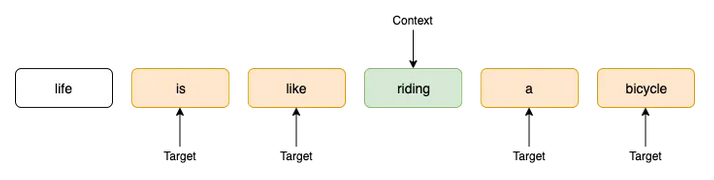
\includegraphics[width=.6\linewidth]{figures/window.png}
\end{figure}

A context word is a word that is ``window\_size'' away from a target word. In this example, window\_size is 2. That means the context words are the 2 words preceding the target word, and the 2 words proceeding the target word.

It creates a context list and a set of targets based upon a hyperparameter window. With a window size of 2 we get the following:

\begin{table}[h]
    \centering
    \begin{tabular}{|c|c|}
        \hline
        \textbf{Context} & \textbf{Target} \\
        \hline
        riding & is \\ 
        riding & like \\
        riding & a \\ 
        riding & bicycle \\ 
        \hline
    \end{tabular}
\end{table}

\subsection{Continuous bag-of-words}

\begin{figure}[H]
    \centering
    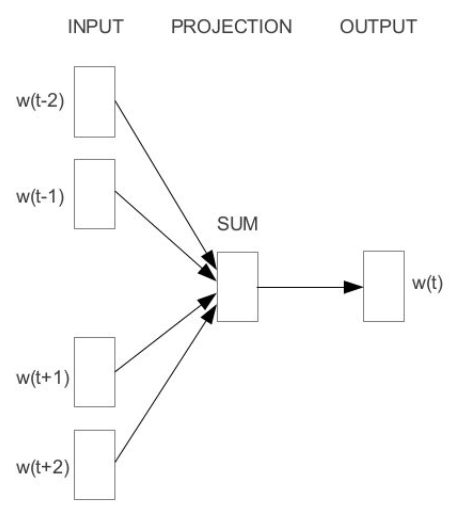
\includegraphics[width=.3\linewidth]{figures/CBOW.png}
\end{figure}

In CBOW, we feed our context words as input to our model. Our model is then optimized to predict what the target word actually is.

\subsection{Skip-gram}

\begin{figure}[H]
    \centering
    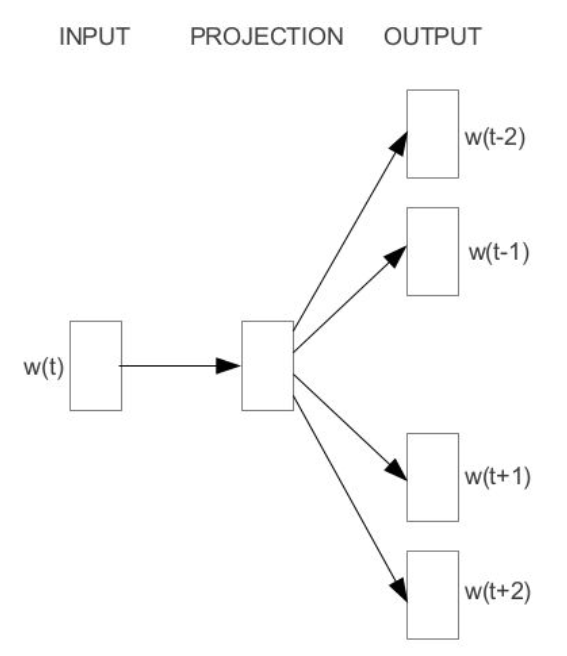
\includegraphics[width=.3\linewidth]{figures/SkipGram.png}
\end{figure}

In Skip-gram~\cite{WordSenseDisambiguation,CBOW-and-skipgram}, we do the opposite. We feed in our target word as input, and the model aims to predict what the context words are

\begin{figure}[H]
    \centering
    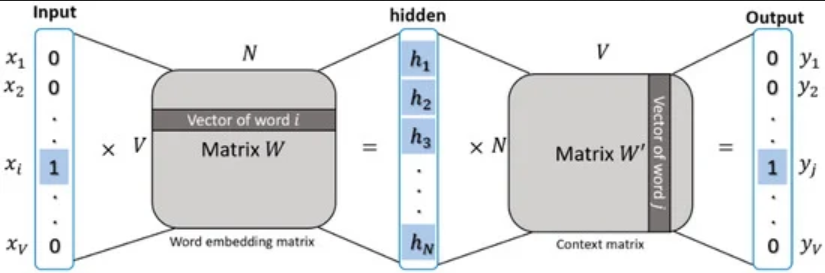
\includegraphics[trim={0 0 0 5px}, clip, width=\linewidth]{figures/SkipGramDetailed.png}
\end{figure}

The architecture is a 2 layered neural network without any non-linearities in between them. 

\begin{enumerate}
    \item Give 1-hot vector of the target word as input x
    \item Map that to the embedding of that target word, using weight matrix W $h=xW$
    
    \begin{figure}
        \centering
        \includegraphics*[width=\linewidth]{figures/one-hot-word-embedding-extraction.png}
    \end{figure}

    \item Map the embedding of the target word to the possible context words, using weight matrix W': $y=hW'$
    \item y has length of the whole vocabulary. Apply softmax to make y into a probability distribution over the whole vocabulary $y'=softmax(y)$
\end{enumerate}

The softmax currently performs a binary classification, whereas we want to find the entire bubble of context words around the word.

\subsubsection{Training}

\begin{figure}[H]
    \centering
    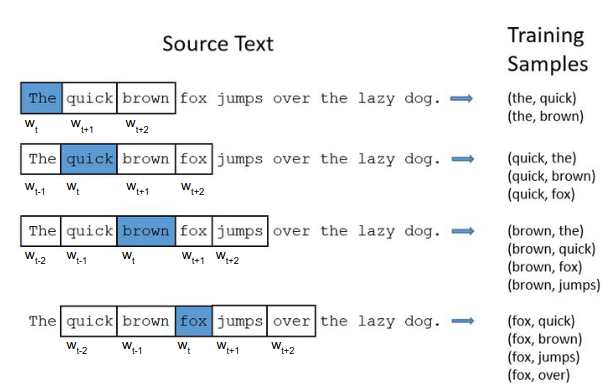
\includegraphics[trim={0 0 0 5px}, clip, width=.8\linewidth]{figures/training-skip-gram.png}
\end{figure}

During training we are building multiple training samples for each target word that we have. More specifically, for each target word, we will normally have $window\_size*2$ training samples; therefore we optimize the model 4 times for each word, each time against a different context word (if it appears multiple times and window is full)

\subsubsection{Loss}

$p(.|.)$ is a probability distribution calculated by softmax.

\begin{equation}
    p(w_{t+j}|w_t) = \frac{\exp({u_{w_{t+j}}^\top h_{w_t}})}{\sum^W_{w'=1} \exp({u_{w'}^\top h_{w_t}})}
    \label{eq:softmax-problem}
\end{equation}

We want to maximise the probability of a context word being correctly predicted for a target word for all words in our target. 

\begin{equation*}
    \max \prod_t \prod_j p(w_{t+j}|w_t)
\end{equation*}

We then turn this into a minimization problem

\begin{equation*}
    \min_\theta - \prod_t \prod_j p(w_{t+j}|w_t;\theta)
\end{equation*}

Multiplying gives the problem of vanishing gradients, therefore we take the logarithm

\begin{equation*}
    \min_\theta - \sum_t \sum_j \log p(w_{t+j}|w_t;\theta)
\end{equation*}

We then explicitly state that we don't calculate a loss over $j=0$ and the loss for one document is the average loss for each word in that document.

\begin{equation*}
    \sum_{-c\leq j \leq c, j \neq 0} \log p(w_{t+j} | w_t ; \theta)
\end{equation*}

Since the loss for the corpus will be this applied over every document in our corpus we have another term

\begin{equation*}
    \frac1 T \sum^T_{t=1} \sum_{-c\leq j \leq c, j \neq 0} \log p(w_{t+j} | w_t ; \theta)
\end{equation*}

All in all, this is actually just a cross-entropy loss function for every target-context training pair we have.

\subsubsection{Using Word Embeddings}

Now that the model is trained, we can separate out the training of the word embeddings and the downstream task we wanted to do. What this means is that we can take our text corpus and train a word2vec algo on it. We can then use one of the learned weights embedding matrix (next slide) to extract out a vector for each word.

\subsubsection{Softmax problem}

In Equation~\ref{eq:softmax-problem} the bottom sum is expensive to compute a single forward pass of the model, we have to sum across the entire corpus vocabulary; this gets inefficient with large vocabularies and large embedding.

We therefore try to approximate softmax instead.

\subsubsection{Negative Sampling}

Use binary classification to distinguish real context words from noise context words. We train a vocabulary number of binary classifiers. That is, each item in the vocabulary has a binary classifier which attempts to predict whether a target word appears in the context of a context word or not.

\begin{equation*}
    \log p(D=1|w_t , w_{t+1}) + k \mathbb{E}_{\tilde{c}\sim P_{noise}}\left[\log p(D=0|w_t, \tilde{c})\right]
\end{equation*}

$p(D=1|w_t, w_{t+1})$ is a binary logistic regression probability of seeing the word $w_t$ in the context $w_{t+1}$.

Approximate expectation by drawing $k$ contrastive context words from a noisy distribution $\tilde{c}$. This comes from randomly drawing from the $P_{noise}$ distribution which could be random sampling or frequency based sampling.

On the left, we have $D=1$, i.e. we want to maximize the probability of correctly predicting that a target word and a TRUE context word appear in context of each other (i.e. predicting a 1 with our binary classifier.)

On the right, we want to maximize the probability of correctly predicting that a target word and a noise word do NOT appear in context of each other ($D=0$).

\textbf{Example:}

\begin{figure}[H]
    \centering
    \includegraphics*[width=.5\linewidth]{figures/skip-gram-negative-sampling-example.png}
\end{figure}

We therefore replace Equation~\ref{eq:softmax-problem} with

\begin{equation}
    p(D=1|w_t, w_{t+1}) = \frac{1}{1 + \exp{-u_{w_{t+1}}^\top h_{w_t}}}\label{eq:sigmoid}
\end{equation}

\subsubsection{Size of k?}

5-20 negative words works well for smaller datasets but 2-5 negative words for larger datasets.

Let's say we had k=5: For a model with weight matrix 300x10K, need to update weights for 1 positive word, plus 5 negative samples. That's 6 output neurons. So 6 * 300 = 1800 weight parameters need to be updated. That is only 0.06\% of the 3M weights in the output layer!

\subsubsection{Noise Distribution}

Random Sampling:

\begin{equation*}
    p(w_i) = \frac 1 {|V|}
\end{equation*}

Frequency Based Sampling:

\begin{equation*}
    p(w_i) = \frac{f(w_i)^{3/4}}{\sum_{w'}f(w')^{3/4}}
\end{equation*}

We sample words from the vocabulary

\section{What can we do with vectors?}

\begin{enumerate}
    \item We can use them to find the most similar other words, given an input word
    \item Analogy Recovery

    Idea: The offset of the vectors should reflect their relation: $a-b \approx c -d \iff d \approx c - a + b$. For example: queen $\approx$ king - man + woman.

    \item Multilingual word embeddings
    
    If we have words from many languages can we a shared embedding space for words that exist within this language?
\end{enumerate}

\printbibliography

\end{document}